\documentclass[12pt,oneside]{book}
\usepackage{times,mathptmx}
\usepackage[pdftex]{graphicx}
\usepackage{calc}
\usepackage{tabularx,ragged2e,booktabs,caption}
\usepackage{array}
\newcolumntype{L}[1]{>{\raggedright\let\newline\\\arraybackslash\hspace{0pt}}m{#1}}
\newcolumntype{C}[1]{>{\centering\let\newline\\\arraybackslash\hspace{0pt}}m{#1}}
\newcolumntype{R}[1]{>{\raggedleft\let\newline\\\arraybackslash\hspace{0pt}}m{#1}}
\usepackage{multirow}
\usepackage{tocloft}
\usepackage{xcolor}
\usepackage{colortbl}
\usepackage{color,soul}
\usepackage{amsmath}
\definecolor{linknavy}{rgb}{0,0,0.50196}
\definecolor{linkred}{rgb}{1,0,0}
\definecolor{linkblue}{rgb}{0,0,1}
\usepackage{float}
\usepackage{graphpap}
\usepackage{rotating}
\usepackage{graphicx}
\usepackage{geometry}
\usepackage{relsize}
\usepackage{ltablex}
\usepackage{longtable}
\usepackage{threeparttable}
\usepackage{lscape}
\usepackage{amssymb}
\usepackage{makeidx} % Create index at end of document
\usepackage[nottoc,notlof,notlot]{tocbibind} % Put the bibliography and index in the ToC
\usepackage{lastpage} % Automatic last page number reference.
\usepackage[T1]{fontenc}
\usepackage{enumerate}
\usepackage{upquote}
\usepackage{moreverb}
\usepackage{xfrac}
\usepackage{cite}
\usepackage{tikz}
\usepackage{fancyhdr}
\usepackage{placeins}
\usepackage{subfig}
% \usepackage{subfig}
% \usepackage{caption}
\usepackage[toc,page]{appendix}
\usepackage{notoccite}
\usepackage{varwidth}

\usepackage{titlesec}
\titleformat{\chapter}[hang] 
{\normalfont\huge\bfseries}{\chaptertitlename\ \thechapter}{1em}{} 
\titlespacing*{\chapter}{0pt}{-30pt}{20pt}

\newcommand{\nopart}{\expandafter\def\csname Parent-1\endcsname{}} % To fix table of contents in pdf.

\usepackage{siunitx}
\sisetup{
    detect-all = true,
    input-decimal-markers = {.},
    input-ignore = {,},
    inter-unit-product = \ensuremath{{}\cdot{}},
    multi-part-units = repeat,
    number-unit-product = \text{~},
    per-mode = fraction,
    separate-uncertainty = true,
}

\usepackage{listings}
\usepackage{textcomp}
\definecolor{lbcolor}{rgb}{0.96,0.96,0.96}

\usepackage[pdftex,
        colorlinks=true,
        urlcolor=linkblue,     % \href{...}{...} external (URL)
        citecolor=linkred,     % citation number colors
        linkcolor=linknavy,    % \ref{...} and \pageref{...}
        pdfproducer={pdflatex},
        pdfpagemode=UseNone,
        bookmarksopen=true,
        plainpages=false,
        verbose]{hyperref}

\setlength{\textwidth}{6.5in}
\setlength{\textheight}{9.0in}
\setlength{\topmargin}{0.in}
\setlength{\headheight}{0.pt}
\setlength{\headsep}{0.in}
\setlength{\parindent}{0.0in}
\setlength{\itemindent}{0.25in}
\setlength{\oddsidemargin}{0.0in}
\setlength{\evensidemargin}{0.0in}
% \setlength{\leftmargini}{\parindent} % Controls the indenting of the "bullets" in a list
\setlength{\cftsecnumwidth}{0.45in}
\setlength{\cftsubsecnumwidth}{0.5in}
\setlength{\cftfignumwidth}{0.45in}
\setlength{\cfttabnumwidth}{0.45in}
\setlength{\parskip}{1em}

\newcommand{\titlesigs}
{
\medskip
\flushright{Underwriters Laboratories Inc.}\\
{\em Terrence Brady, President}
\medskip
\flushright{UL Firefighter Safety Research Institute\\
{\em Stephen Kerber, Director} \\
\hspace{1in} \\
}
}

\newcommand{\headerB}[1]{
\flushleft{
\fontsize{28}{33.6}\selectfont
\bf{#1}
}
}

\newcommand{\headerC}[1]{
\vspace{.5in}
\flushright{\fontsize{14}{16.8}\selectfont
#1}
}

% \newcolumntype{L}{>{\centering\arraybackslash}m{4cm}}

\floatstyle{boxed}
\newfloat{notebox}{H}{lon}
\newfloat{warning}{H}{low}

\newenvironment{conditions}
  {\par\vspace{\abovedisplayskip}\noindent\begin{tabular}{>{$}l<{$} @{${}={}$} l}}
  {\end{tabular}\par\vspace{\belowdisplayskip}}


% Rename chapter headings
\renewcommand{\chaptername}{}
\renewcommand{\bibname}{References}

\usepackage{fancyhdr}
\pagestyle{fancy}
\lhead{}
\rhead{}
\chead{}
\renewcommand{\headrulewidth}{0pt}


% COMMENT TO REMOVE WATERMARK
\usepackage{draftwatermark}
\SetWatermarkText{DRAFT}
\SetWatermarkScale{1}

\begin{document}
\pagenumbering{gobble}
\bibliographystyle{unsrt}
	
\begin{minipage}[t][9in][s]{6.25in}

\headerB{
Post-Fire Exposures: Examination of Hot, Warm and Cold Scenes  \\
}

\normalsize
\headerC{
	\flushleft{
	Gavin P. Horn \\
	Daniel Madrzykowski \\

\vspace{0.2in}
	UL Firefighter Safety Research Institute \\
	Columbia, MD 20145 \\
	\vspace*{2\baselineskip}
	

	Summer Neumann     \\

\vspace{0.2in}
	UL Environment \& Sustainability \\
	Lake Forest, CA 92630  \\
	\vspace*{2\baselineskip}
	}
}
	\vfill

\begin{flushright}
\begin{minipage}{0.5\textwidth}
\includegraphics[width=\textwidth]{UnderwritersLaboratories_TM} \\ 
\end{minipage} \hfill
\begin{minipage}{0.25\textwidth}
\includegraphics[width=2.0in]{FSRI_GraphicShield} \\ 
\end{minipage}
\end{flushright}

\scriptsize
\flushright{Copyright 2020. \textcopyright Underwriters Laboratories Inc. All rights reserved. UL and the UL logo are trademarks of UL LLC}
\end{minipage}

\newpage
\hspace{5in}
\newpage

\begin{minipage}[t][9in][s]{6.25in}
\pagenumbering{gobble}

\headerB{
Post-Fire Exposures: Examination of Hot, Warm and Cold Scenes \\
}

\headerC{
	\flushleft{
	Gavin P. Horn \\
	Daniel Madrzykowski \\

\vspace{0.2in}
	UL Firefighter Safety Research Institute \\
	Columbia, MD 20145 \\
	\vspace*{2\baselineskip}
	

	Summer Neumann     \\

\vspace{0.2in}
	UL Environment \& Sustainability \\
	Lake Forest, CA 92630  \\
	\vspace*{2\baselineskip}
	}
}
	\vfill

\begin{flushright}
\begin{minipage}{0.5\textwidth}
\includegraphics[width=\textwidth]{UnderwritersLaboratories_TM} \\ 
\end{minipage} \hfill
\begin{minipage}{0.25\textwidth}
\includegraphics[width=2.0in]{FSRI_GraphicShield} \\ 
\end{minipage}
\end{flushright}
\titlesigs

\scriptsize
\flushright{Copyright 2020. \textcopyright Underwriters Laboratories Inc. All rights reserved. UL and the UL logo are trademarks of UL LLC}
\end{minipage}

\newpage

\begin{minipage}[t][9in][s]{6.25in}

\flushleft{In no event shall UL be responsible to anyone for whatever use or non-use is made of the information contained in this Report and in no event shall UL, its employees, or its agents incur any obligation or liability for damages including, but not limited to, consequential damage arising out of or in connection  with the use or inability to use the information contained in this Report. Information conveyed by this Report applies only to the specimens actually involved in these tests. UL has not established a factory Follow-Up Service Program to determine the conformance of subsequently produced material, nor has any provision been made to apply any registered mark of UL to such material. The issuance of this Report in no way implies Listing, Classification or Recognition by UL and does not authorize the use of UL Listing, Classification or Recognition Marks or other reference to UL on or in connection with the product or system.
}

\vspace{3in}
\vfill
\hspace{1in}

\end{minipage}

\newpage

\frontmatter

\pagestyle{plain}
\pagenumbering{roman}

\cleardoublepage
\phantomsection
\tableofcontents

\cleardoublepage
\phantomsection
\addcontentsline{toc}{chapter}{List of Figures}
\listoffigures

\cleardoublepage
\phantomsection
\addcontentsline{toc}{chapter}{List of Tables}
\listoftables

\chapter{List of Abbreviations}

\begin{tabbing}
\hspace{1.5in} \= \\
ABS 	    \> arylonitrile butadiene styrene \\
ATF 	    \> Bureau of Alcohol, Tobacco, and Firearms \\
BTEX 	    \> benzene, toluene, ethylbenzene and xylene \\
EPS 	    \> expanded polystyrene  \\
HDPE 	    \> high-density polyethylene \\
HHE 	    \> Health Hazard Evaluation \\
IARC 	    \> International Agency for Research on Cancer \\
LDPE 	    \> low-density polyethylene  \\
MDF 	    \> medium density fiberboard \\
NIOSH 	    \> National Institute for Occupational Safety and Health \\
NIST 	    \> National Institute for Standards and Technology \\
OEL 	    \> occupational exposure limit \\
PAH 	    \> polycylic aromatic hydrocarbon \\
PC 	  	  	\> polycarbonate  \\
PET 	    \> polyethylene terephthalate \\
PFI 	    \> police fire investigators \\
PLA 	    \> polylactic acid \\
PMMA 	    \> polymethyl methacrylate \\
PPE 	    \> personal protective equipment \\
PU 	  	  	\> polyurethane   \\
PVC 	    \> polyvinyl chloride \\
SCBA 	    \> self contained breathing appratus \\
STEL 	    \> short term exposure limit \\
TWA 	    \> time weighted average \\
UL 	    	\> Underwriters Laboratories \\
UL 	    	\> Underwriters Laboratories \\
UL FSRI 	\> UL Firefighter Safety Research Institute \\
VOC 	    \> volatile organic compound \\
\end{tabbing}

\mainmatter

\chapter*{Acknowledgments}
\pagenumbering{gobble}

\begin{table}[!ht]
	\centering
	\caption*{Huge thanks to the following for their support!}
	\begin{tabular}{ll}
		\toprule[1.5pt]
		Name & Role \\ 
		\midrule
		Sameual Horner		 & Lead field data collection \\
		Mark Carpenter		 & Scientific support \\
		Nelson Tirado		 & Field data collectionsupport \\
		 
		\bottomrule[1.25pt]
	\end{tabular}
\end{table}

\newpage

\chapter*{Abstract}

\newpage
\chapter{Introduction}
\label{chap:intro}
\pagenumbering{arabic}
\setcounter{page}{1}

The fire service has witnessed growing evidence of occupational exposures and an overall increased cancer risk compared to the general population. While much of this research has focused on structural firefighters, potential risks for post-fire scnene investigators have not been fully characterized. Fire investigators’ occupational exposures are likely lower than structural firefighters, as they are generally active in the fire building after extinquishment.  The timeframe for active investigation can range from immediate post supprsssion (before or during overhaul) to several days after fire suppression has been completed. Cause and origin investigators are likely to be working on scene for several hours, possibly over multiple days. Oftentimes, due in part to a lack of active fire and challenges in completing important documentation tasks, the use of PPE among fire investigators is not consistent, potentially increasing their susceptibility to carcinogenic exposures.  The concentration of chemical exposures for fire investigators is expected to be lower than structural firefighters, but the type of chemicals fire investigators are exposed to are expected to be similar to what is found on the fireground. The IAAI Fire Investigator Health and Safety Best Practices guidelines recommends fire investigators monitor for carbon monoxide and hydrogen cyanide during the incident. However, many other harmful substances found during overhaul are likely to exist during the fire investigation and may not follow the same trends as the more easily  monitored gases. <<cite Gainey et al 2019 and TVFR report 2011>>.  

It has been well documnted that today's structure fires can produce hundreds of compounds including carcinogens like aldehydes, polycyclic aromatic hydrocarbons (PAHs), volatile organic compuonds (VOCs) particularly benzene, and high levels of airbore particulate.(1-4) Epidemiological studies have documented an increased risk for certain types of cancer,(5-8) and the International Agency for Research on Cancer (IARC) classified firefighters’ occupational exposure to be possibly carcinogenic to humans (Group 2B).(9) Occupational exposure risks during fire responses are often characterized as a high magnitude but for a relatively short duration. Heavy insulating firefighter PPE and self-contained breathing appratus (SCBA) are well suited for these risks and compliance with PPE usage is common given the known risks. However, due to the enxtended duration of overhaul and investigation, PPE usage is not as consistent. And concentrations of PAHs and benzene during overhaul, after the fire has been extinguished, have  been found to exceed short-term exposure limits.(2,4) 

Fire investigators arrive on the fire scene after the fire is extinguished and the IDLH hazards are mitigated.  However, there are still sufficient physical and chemical hazards at the fire scene. 
 <<Fire investigator examining a scene several days after the fire, when the air seems safe.>>

The IAAI has defined catagories of fire scenes based on the post-fire extinguishment time and has recommended PPE protection for each time period based on the potential hazard that may exist~\cite{IAAI:2020}.   

\begin{enumerate}
\item HOT SCENE A: A fire scene where the fire has been extinguished, but overhaul has not yet commenced or is in progress.

\item HOT SCENE B: A fire scene that has been fully extinguished/overhauled for less than two hours.

\item  WARM SCENE: A fire scene that has been fully extinguished at least two hours but for less than 72 hours. 

\item COLD SCENE: A fire scene that has been fully extinguished for at least 72 hours and not generating detectable or visible dust, fumes, mists, particulates, gases, vapors or aerosols.

\end{enumerate}

\section{Post-fire Investigator focused studies}
Suprisingly few studies have focused on these time periods, specific to fire investigators.  In 1998, the National Institute for Occupational Safety and Health (NIOSH) released a report based on a health hazard evaluation (HHE) request from the Bureau of Alcohol, Tobacco, and Firearms (ATF) << reference Kinnes and Hine, 1992>>. Environmental monitoring, including total and respirable dust, metals, hydrogen cyanide, inorganic acids, aldehydes, PAHs, and VOCs, was performed during the investigation of two house fires in metropolitan Washington, D.C., and Prince George's County, Maryland, and three staged fires at the Fort Belvoir military base in Alexandria, Virginia. Low concentrations were found for most of the analytes, though formaldehyde was detected at concentrations up to 0.18 ppm.Total and respirable dust were also detected at time-weighted average (TWA) concentrations up to 5.3 and 1.3 mg/m3, respectively with peak total dust concentrations up to 30 mg/m3. The authors suggest that excessive dust concentrations were encountered for short durations during some activities. Importantly, it was noted that several fire investigators, who did not wear respiratory protection, experienced both eye and respiratory irritation during these investigations. 

In 2013, Fent et al reported on the Evaluation of Dermal Exposure to Polycyclic Aromatic Hydrocarbons in Fire Fighters as part of an HHE.  This effort included some monitoring of envirnonmental conditionns during Overhaul and Investigation (approximately the time period as Hot Zone A and Hot Zone B, respectively) as well as suppression. PAH concentrations were highest during the fire phase, then dropped quickly during the subsequent overhaul and investigation phases. The overhaul concentrations were 7–280 times higher than the background concentrations, including one scenario where air concentratione exceeded the ACGIH excursion limit for coal tar pitch volatiles. The investigation concentrations were 7–11 times higher than the background concentrations for two of the six scenarios (none exceeded ACGIH excursion limit for coal tar pitch volatiles). In general, VOC concentrations were higher during overhaul than background or investigation phases, though measurable benzene, styrene, toluene and carbon disulfide were reported during the investigation period. All concentrations of these VOCs were well below their short term exposure limits (STELs). Particulate concentration levels remained exceeded instrumentation ranges during the fire period and remained elevated compared to background levels through the overhaul phase of each burn and during the investigation phase of one scenario. Some materials were still smoldering during the investigation phase of this burn, though no overhaul of the physical environment (dropping and removing drywall, moving burnt furnshings). Fent et al (2013) note that air measurements during overhaul andinvestigation may underestimate typical fire fighters exposures because the burn structures were relatively small and well-ventilated, which allowed heat and contaminants to dissipate quickly. In addition, they did not measure air concentrations of a variety of chemicals including aldehydes and cyanides.


Recently, as part of a larger study, Sjostrom et al (2019) assessed  exposure to PAHs, VOCs, and particles on nine police forensic investigators (PFIs) investigating the aftermath of live fire events in Sweden. These nine participants responded to five different fires in a wide range of settings (a cottage, an apartment building, an office, an antique store, and a warehouse) and various timeframes (from within 12 h of the fire to 5 days after the fire). PFIs were found to be exposed to several hazardous compounds during their work, particularly napththalene (mean of 4.58 microg/m3 with a range of 0.12-76.9 microg/m3), benzene (mean of 19.3 microg/m3 with a range of 1.8-78.3 microg/m3) and total dust (mean of 176 microg/m3 with a range of 70-314 microg/m3). These exposures were substantially higher than urban background levels but well below Swedish occupational exposure limits (OELs).


\section{Post-fire Overhaul focused studies}
In addition to fire investigator focused data collection, addditional studies have increased our understanding of environmental conditions and occupational risks that may be encountered while firefighters are conducting the post-suppression overhaul process (Bolstad-Johnson et al 2000; TVFR 2011; Fent et al 2013,2018, Gainey et al 2019?). These environments are likely similar to that which fire investigators may experience when conducting early work in a Hot scene A.

Bolstad-Johnson et al (2000) conducte an air monitoring study with Phoenix firefighters during the overhaul phase of 25 structure fires. Personal samples were collected for aldehydes, BTEX, hydrochloric acid, polynuclear aromatic hydrocarbons (PNA - another name for PAHs?), respirable dust, and hydrogen cyanide (HCN). Area samples were collected for asbestos, metals
(Cd, Cr, Pb), and total dust. Published ceiling values were exceeded for acrolein (American Conference of Governmental Industrial Hygienists [ACGIHT] 0.1 ppm) at 1 fire; CO (National Institute for Occupational Safety and Health [NIOSH] 200 ppm) at 5 fires; formaldehyde (NIOSH 0.1 ppm) at 22 fires; and glutaraldehyde (ACGIH 0.05 ppm) at 5 fires. In addition, the following exceeded published short-term exposure limit values: benzene (NIOSH 1 ppm) at two fires, NO2 (NIOSH 1 ppm) at two fires, and SO2 (ACGIH 5 ppm) at five fires. 10-min average CO concentrations did not predict concentrations of other products of combustion, suggesting that CO should not be used as an indicator gas for other contaminants found in this atmosphere.


Weiss and Miller (2011) measured airborne concentrations of several chemicals during the overhaul phase at thirty-eight actual fire responses including 23 single family residences, 5 apartment residences, 2 barn fires, 3 commercial/industrial structures, 4 recreational vehicles, and 1 adult foster care home.... One of their primary conclusions supports the findings of Bolstad-Johnson et al (2000) in that CO levels did not predict other chemicals’ presence or concentrations at fire scenes. While the presence of some chemicals seems to predict that of others, there was no specific chemical that will reliably predict them all.  As part of the data analysis, chemical levels were recorded up to 65 minutes after the fire was knocked down. The authors found a natural dissipation of chemical levels over the first 45 minutes post knock down. After 1 hour, most products had completely dissipated.

Fent et al (2017) characterized area and personal air concentrations of combustion byproducts produced during controlled residential fires with furnishings common in 21st century single family structures. Area and personal air measurements were collected during active fire and overhaul. Sampled compounds included PAHs, VOCs, hydrogen cyanide (HCN), and particulate. Personal air concentrations of total PAHs and benzene measured from some overhaul firefighters exceeded exposure limits.

\section{Objectives}

To improve the health and safety of fire investigators through understanding the risk for solid phase and vapor phase chemical exposures at the post-fire scene.  These experiments will characterize air-borne contaminants that may be encountered while investigating a residential fire scene and how these contaminants may evolve in the days following the fire, from within an hour after fire extinguishment to 5 days after the fire.          


\chapter{Measurement Approach}

Area monitoring devices are set up either in the kitchen/living room area or a bedroom depending on the area of origin of the fire.  Samples for polycyclic aromatic hydrocarbons (PAHs), aldehydes, carbon monoxide, hydrogen sulfide, hydrogen cyanide, volatile organic compounds (VOCs -particularly benzene, toluene, ethylbenzene and xylene (BTEX)), fibers and a variety of metals are being collected.  

\section{Instrumentation}
\label{sec:instrument}

\subsection{Measurement Locations}
\label{subsec:measure_locs}

\subsection{Measurement Uncertainty}
\label{subsec:uncertainty}

There are different components of uncertainty in the measured values reported in this document, specifically gas temperature, total heat flux, pressure, gas velocity, gas concentration, heat release rate, length, mass, structure leakage, and water flow rate. Uncertainties are grouped into two categories according to the method used to estimate them. Type A uncertainties are those evaluated by statistical methods, and Type B are those evaluated by other means~\cite{Taylor&Kuyatt:1994}. Type B analysis of systematic uncertainties involves estimating the upper ($+$~a) and lower ($-$~a) limits for the quantity in question such that the probability that the value would be in the interval ($\pm$~a) is essentially 100~\%. After estimating uncertainties by either Type A or B analysis, the uncertainties can be combined in quadrature to yield the combined standard uncertainty. Multiplying this combined standard uncertainty by a coverage factor of two results in an expanded uncertainty with a 95~\% confidence interval (2$\sigma$). For some components, such as the zero and calibration elements, uncertainties were derived from referenced instrument specifications. For other components, referenced research results and past experience with the instruments provided input for the uncertainty determination.

\subsubsection*{Length}
Length measurements, such as the room dimensions and instrumentation locations, were made with either a hand held laser measurement device having an accuracy of 0.25~in. ($\pm$~6.0~mm) over a range of 2~ft (0.6~m) to 50~ft (15.2~m)~\cite{StanleyTools} or $\pm$~0.02~in. ($\pm$~0.51~mm) resolution steel measuring tapes manufactured in compliance with NIST Manual 44~\cite{Butcher:2012}, which specifies a tolerance of $\pm$~0.06~in. ($\pm$~1.5~mm) for 30~ft (9.1~m) tapes and $\pm$~0.25~in. ($\pm$~6.4~mm) for 100~ft (30.5~m) tapes. These uncertainties are all well within the precision of the reported dimensions, which are typically rounded to the nearest inch. Some issues, such as levelness of the device and ``soft'' edges on upholstered furniture, result in an estimated expanded uncertainty of $\pm$~1.0~\% for reported length measurements.

\subsubsection*{Mass}
The load cell used to weigh the fuels prior to the experiments had a range of 0~lb (0~kg) to 441~lb (200~kg) with a resolution of 0.11~lb (0.05~kg) and a calibration uncertainty within 1~\%~\cite{Ohaus:2000}. The total expanded uncertainty for the fuel weights measured by the load cell that are presented in this report is estimated to be less than $\pm$~5~\%.

\subsubsection*{Structure Leakage} 
To characterize ventilation within the structure, an air leakage measurement system (Model~5101) was used to measure the amount of leakage associated with the training prop before each test~\cite{retrotec:leakage}. \textit{ASTM~E779-10, Standard Test Method for Determining Air Leakage Rate by Fan Pressurization} was followed to determine the air leakage rate of the prop before each experiment~\cite{astm_e779}. The measured leakage rates were recorded in units of air changes per hour at 50~Pa (ACPH50). Retrotec, the manufacturer of the leakage measurement system, reports an accuracy of $\pm$~5~\% for the system.

\subsubsection*{Water Flow Rate}
Water flow rate was measured with a 1.5~in. (3.8~cm) diameter electromagnetic flow meter from Badger Meter, Inc. (Model~M2000). The meter consisted of stainless steel pipe lined with a non-conductive material. Energized coils on the outside of the non-conductive material imposed a magnetic field across the pipe, and when the conductive fluid (water) flowed across the magnetic field, a voltage proportional to flow velocity was produced. The manufacturer reports a $\pm$~0.25~\% calibration uncertainty for the accuracy of the measurement~\cite{Badger:2015}.

\subsubsection*{Airborne Contaminants}
\hl{Will depend upon technique used to measure each class of chemicals and particulate dimensions.} 


\begin{table}[!ht]
	\centering
	\caption{Airborne contaminant experimental measurements}
	\begin{tabular}{lccc}
		\toprule[1.5pt]
		Compound & Method & Media & Pump \\
		\midrule
		PAH   				& AfPS GS 2019:01 PAK   & OVS-7     		& 1 Lpm     \\
		VOC    				& TO-17     			& Carbopack/Carbomet& 0.2? Lpm    \\
		Aldehydes   	 	& ASTM D5197		    & XAD-2?   			& 0.2 Lpm    \\
		Fibers    			& NIOSH 7400B      		& filter cassette 	& 0.5-16 Lpm   \\
		Hydrogen Sulfide  	& NIOSH 6103		    & filter/charcoal	& 0.2? Lpm     \\
		Hydrogen Cyanide   	& NIOSH 6010		    & Soda lime			& 0.2 Lpm    \\
		Particulate   		& Direct Read     		& TSI Dustrak 		& ?? Lpm    \\
		\bottomrule[1.25pt]
	\end{tabular}
\end{table}
The estimated minimum detectable concentration of PAHs, HCN, and benzene  is  0.0021 mg/m3.
The estimated minimum detectable concentration of acid gas concentrations is 0.175 mg/m3.


\chapter{Experimental Configuration}
\label{chap:exp_config}

\section{Experimental Structure}

Two identical, purpose-built residential structures were constructed on the grounds of the Delaware County Emergency Services Training Center (ESTC) in Sharon Hill, Pennsylvania. The design of the structures, fuel loads, and set of experiments were planned during a workshop with the technical panel assembled for a related study (DHS Size Up, Search and Rescue).  These test structures were approximately 1600~ft$^2$ single-story, four bedroom, 2 bathroom ranch homes equipment with an heating, ventilation, and air conditioning (HVAC) system typical to the northeastern region of the United States. Figure~\ref{fig:Floor_Plan} shows the structure floor plan.

\begin{figure}[!htb]
	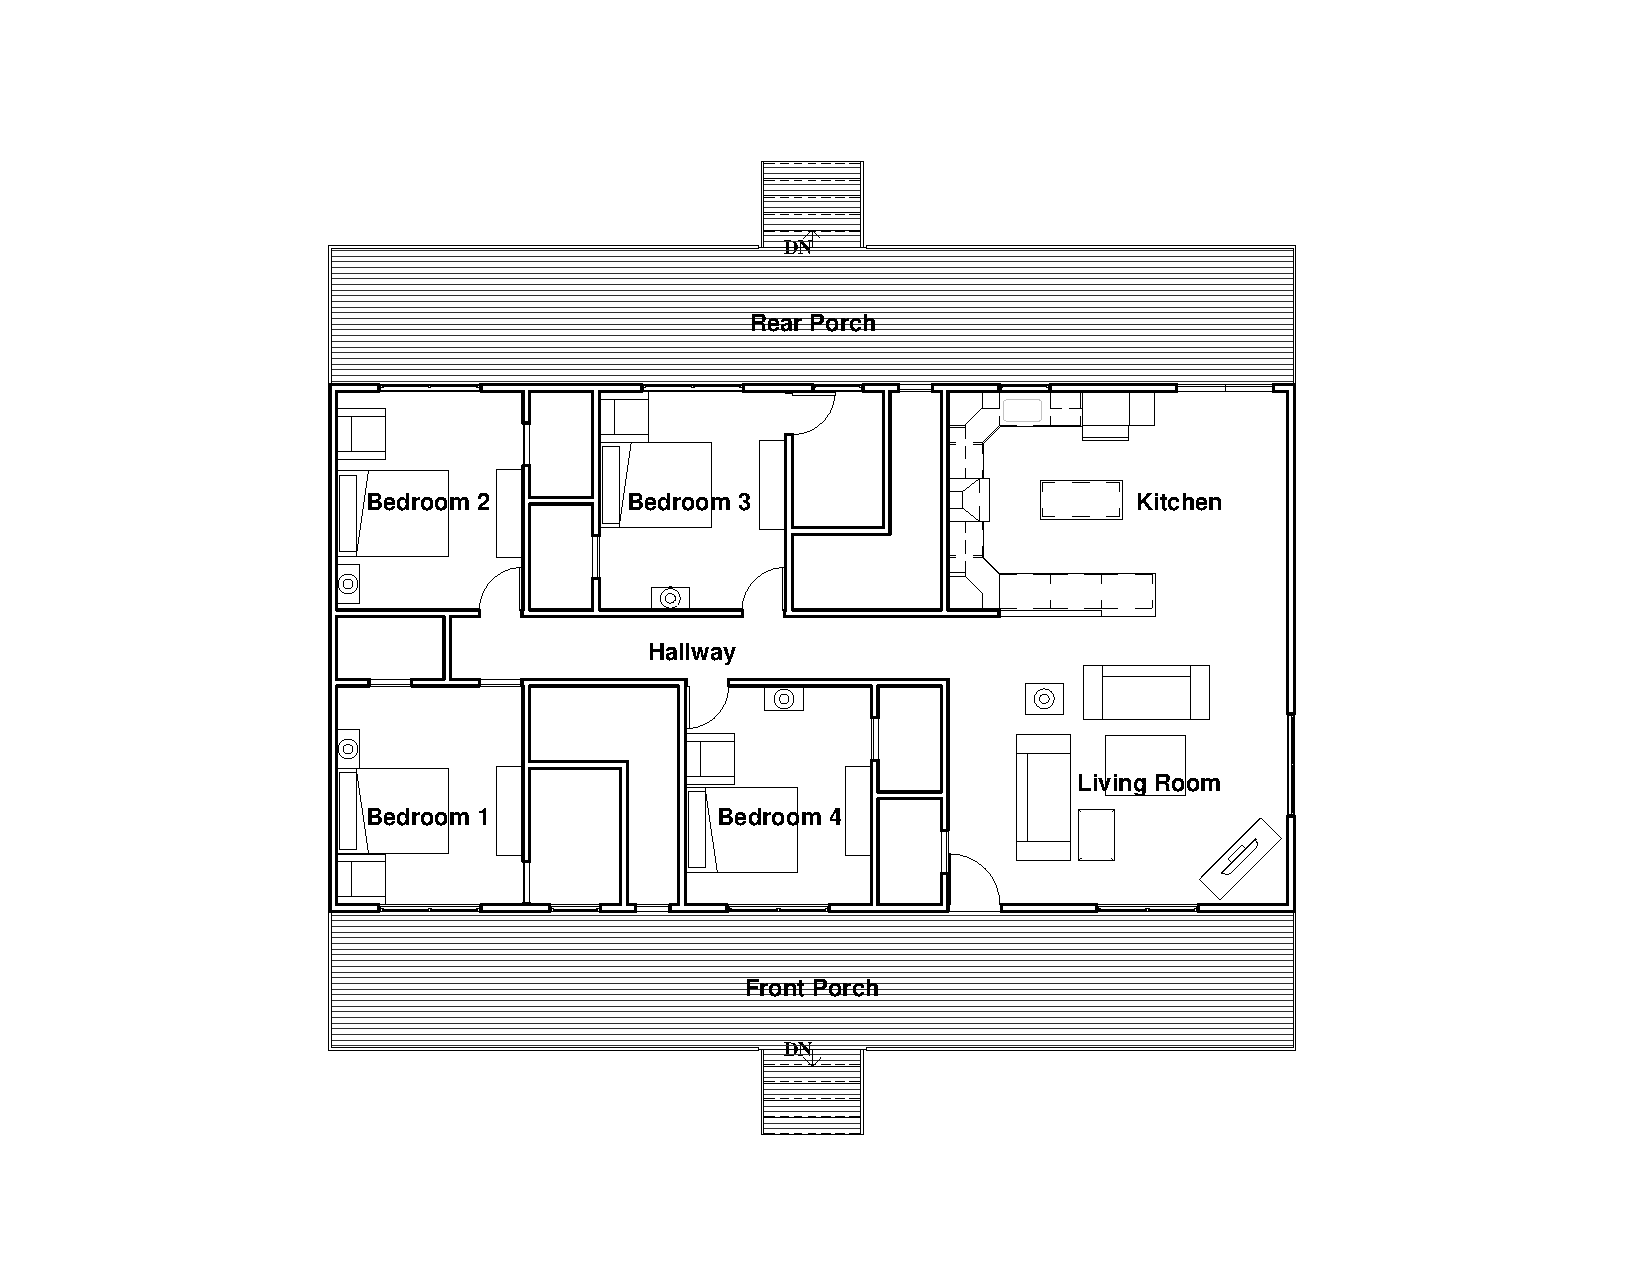
\includegraphics[width=1.1\linewidth]{../06_Figures/Search_Bldg_3}
	\caption{Experimental structure layout}
	\label{fig:Floor_Plan}
\end{figure}


\section{Structure Contents}

Prior to ignition, the structure was fully furnished to represent fuel load conditions typical to a residential structure. This included furnishing each of the four bedrooms, the two bathrooms, the kitchen, and living room. The overall arrangement and dimensions of a representative furnished apartment is presented in Figure~XX


The furnishings were measured and weighed, and where possible, the base materials used in their construction were determined and documented. The furnishings specific to the kitchen, living room and bedroom fuel packages are presented in Section~\ref{sec:kit_fuel}--\ref{sec:br_fuel} along with representative photographs.

\subsection{Kitchen}
\label{sec:kit_fuel}

\begin{table}[!ht]
	\centering
	\caption{Table of Kitchen Furnishings}
	\label{tab:BRFuel}
	\begin{tabular}{llll}
		\toprule[1.5pt]
		Item 				& Dimensions (in) 	& Materials 										& Mass (kg)  \\
		\midrule
		36 in Wall Cabinet 	&  36 x 12 x 36 H	& MDF with wood veneer and door frames 				& 25.35 \\
		Corner Wall Cabinet &  24 x 12 x 36 H	& MDF with wood veneer and door frames   			& 27.10 \\
		30 in Wall Cabinet  &  30 x 12 x 24 H	& MDF with wood veneer and door frames 				& 14.05 \\
		21 in Wall Cabinet  &  21 x 12 x 36 H   & MDF with wood veneer and door frames              & 15.7  \\
		12 in Wall Cabinet  &  12 x 12 x 36 H 	& MDF with wood veneer and door frames 				& 12.30  \\	
		33 in Wall Cabinet 	&  33 x 12 x 18 H	& MDF with wood veneer and door frames 				& 10.40   \\
		36 in Base Cabinet	&  36 x 25 x 34.5 H	& Plywood with wood veneer and door frames			& 30.35    \\	
		24 in Base Cabinet	&  24 x 25 x 34.5 H	& Plywood with wood veneer and door frames			& 19.90    \\
		27 in Base Cabinet	&  27 x 25 x 34.5 H	& Plywood with wood veneer and door frames			& 21.55   \\
		Corner Base Cabinet	&  30 x 30 x 34.5 H	& Plywood with wood veneer and door frames			& 26.5    \\
		36 in Base Cabinet	&  36 x 25 x 34.5 H	& Plywood with wood veneer and door frames			& 21.3    \\
		Tall Cabinet		&  18 x 24 x 90 H	& Plywood with wood veneer and door frames			& 35.30    \\
		Counter Top			&  27 x 57 x 		& Plastic Laminate over particle board          	& 17.6    \\
		Range Hood/Fan		&   x  x 			& Steel Nylon										&      \\
		Fill Panel			&  96 x 24 x 1		& Veneer over Plywood 								& 12.20  \\
		Fill Board		 	&  48 x 96 x 0.25  	& Veneer over fiberboard    						& 13.25   \\
		Composite Flooring	&   0.17 thick 		& IXPE foam, vinyl, PU wear layer					&	0.675 kg/ft2  \\
		Table				& 45 x 24 x 30		& Vinyl covered MDF with wood legs					& 	15.85 \\
		Chair (2)			& 22.5 x 19.5 x 39  & Wood Frame, PU foam, PE Fabric 					&  16.2  \\
		Picture 			& 30 x 24 x 1		& Canvas, Styrene over MDF frame, cardboard 		&  1.45  \\
		Refrigerator		&  x  x             & Steel, rigid foam, plastic liner					&        \\
		Range 				&  x   x 			& Steel, plastic 									&        \\
		\bottomrule[1.25pt]
	\end{tabular}
\end{table}

\begin{table}[!ht]
	\centering
	\caption{Table of Kitchen Plastics. Dimensions are provided for single items.  Mass is provided for the total number of items.}
	\label{tab:KitPlastics}
	\begin{tabular}{llll}
		\toprule[1.5pt]
		Item 				& Dimensions (in) 	& Materials 										& Mass (g)  \\
		\midrule
		Water Bottles (20) 	& 2.5 dia. x 8  	& PET												&  180      \\
		Milk jugs (2)     	& 6 x 6 x 10  		& HDPE											   	&   65      \\
		Recycling Bin  		& 26 x 16 x 15	    & LDPE						  						& 2120     \\
		Two Gallon Bin  	& 8.75 x 9.5 x 9	& PC 							 					&  750     \\	
		7 Piece Utensils	& 3.5 x 12.5 x 0.5	& Nylon											 	&  340   \\	
		Small Food Canister	& 6.5 x 4.75 x 8.75	& Polypropylene							  			&  187   \\
		Small Lid			& 7 x 5 x 2			& HDPE												&   75  \\
		Medium Food Canister& 7.5 x 3.6 x 11 	& Polypropylene 									&  227   \\
		Medium Lid			& 7.9 x 4 x  2		& HDPE												&   60    \\
		Large Food Canister	& 9.1 x 5.25 x 9	& Polypropylene										&  400	 \\
		Large Lid 			& 9.75 x 5.3 x 2	& HDPE 												&   98    \\
		Recipe holders (2)	& 8.6 x 3.25 x 11   & PMMA												&  640	 \\
		Coffeemaker Body	& 8 x 10.5 x 12.5	& ABS 												& 1060   \\
		Cups (25)			& 20 oz				& EPS												&  125   \\
        Cups (50)			& 20 oz				& PLA  												&  380   \\
        Pipe                & 1.5 in OD x 18 in & PVC 												&  360   \\
        Electrical Box	    & 4.3 x 3.5 x 6.5	& PVC 												&  174  \\
        Outlet (2)			& 2.7 x 1.3 x 1.0	& PVC												&  103   \\
        Outlet Cover Plate  & 5.4 x 5.3 x 0.3	& PVC  												&   42   \\
        14-2 NM Cable 		& 60 long			& PVC over copper									&  130  \\
		\bottomrule[1.25pt]
	\end{tabular}
\end{table}

Kitchen ignition set-up   




\subsection{Living Room}
\label{sec:lr_fuel}

\begin{table}[!ht]
	\centering
	\caption{Table of Living Room Contents}
	\label{tab:BRFuel}
	\begin{tabular}{llll}
		\toprule[1.5pt]
		Item 				& Dimensions (in) 	& Materials 										& Mass (kg)  \\
		\midrule
		Sofa (2) 		  	& 87 x 36 x 34  	& Fabric PE, Fill PU foam \& PE, Frame Eng. Wood	& 52.6 53.0 \\
		Ottoman     		& 29 x 16 x 23 		& Fabric PE, Fill PU foam \& PE, Frame Eng. Wood   	& 8.45       \\
		Coffee Table   		& 55 x 42 x 16.5	& Vinyl over particle board  						& 40.60     \\
		End Table      		& 26 x 22 x 26 		& Vinyl over particle board  leg? 					& 27.85     \\	
		TV Stand	 		& 50 x 20 x 30 		& Shell 52~\% PE \& 48~\% cotton, Fill 100~\%PE 	& 56.55     \\	
		TV 					& 38 x 22 x 4		& Shell ?										 	& 7.9       \\
		Lamp 				& 12 dia x 25h		& Body Cast Vinyl, Shade Fabric over plasticfilm	& 1.45      \\
		Curtains(2 pair) 	& 84 x 84 			& 100~\% PE 										& 2.3       \\
		Carpet				&  Pile Height		& Fiber 100~\% PET, PP Backing with Latex			& 0.14 kg/sq ft \\
		Padding				&  0.44	thick   	& PU rebond foam									& 0.29 kg/sq ft	\\
		\bottomrule[1.25pt]
	\end{tabular}
\end{table}



\subsection{Bedroom}
\label{sec:br_fuel}

The bedroom fire scenarios utilized a consitent fuel load that consisted of a queen mattress set with foam mattress topper, a dresser, a night stand, lamp, chair window curtains, and a wall painting as well as being fully carpeted with padding. Table~\ref{tab:BRFuel} shows the size, material composition, and mass of each of the items that comprised a bedroom fuel load for each experiment. Figure~\ref{fig:br_fuel} shows the typical bedroom fuel load. 

Other stuff -- interior doors moldings,  vinyl window frames, Llama paintings, 

\begin{table}[!ht]
	\centering
	\caption{Table of Bedroom Contents}
	\label{tab:BRFuel}
	\begin{tabular}{llll}
		\toprule[1.5pt]
		Item 				& Dimensions (in) 	& Materials 										& Mass (kg)  \\
		\midrule
		Mattress Topper  	& 75 x 58 x 4  		& PU foam  											& 6.85    \\
		Mattress     		& 79 x 59 x 12  	& 90~\% PU foam, 10~\% Blended rayon \& polyester   & 30.1    \\
		Foundation   		& 79 x 59 x 9  		& PE padded fabric over wood  						& 15.45   \\
		Bedding      		& Queen size 		& 100~\% PE     									& 3.5     \\	
		Pillow(2)	 		& 27 x 17 x 4 		& Shell 52~\% PE \& 48~\% cotton, Fill 100~\%PE 	& 1.2     \\	
		Chair				& 32 x 26 x 34		& Fabric 100~\% PE, Fill PU foam \& PE  			& 22.0    \\
		Dresser				& 62 x 17 x 36  	& Vinyl over particle board w/cardboard back		& 49.55   \\
		Nightstand			& 27 x 15.5 x 27	& Vinyl over particle board w/cardboard back		& 15.9    \\
		Lamp 				& 12 x 12 x 25		& Body Cast Vinyl, Shade Fabric over plasticfilm	& 1.45    \\
		Painting			& 30 x 24 x 2		& Frame, Styrene over MDF, Canvas					& 1.45    \\
		Curtains(pair) 		& 84 x 84 			& 100~\% PE 										& 1.15    \\
		Carpet				& 144 x 144 x 		& Fiber 100~\% PET, Backing PP and Latex			& 20.3    \\
		Padding				& 144 x 144 x 0.44	& PU rebond foam									& 19.1	  \\
		\bottomrule[1.25pt]
	\end{tabular}
\end{table}



\FloatBarrier

\begin{figure}[H]
	\centering
	\subfloat[View from Windows Toward Door\label{fig:br_fuel1}]{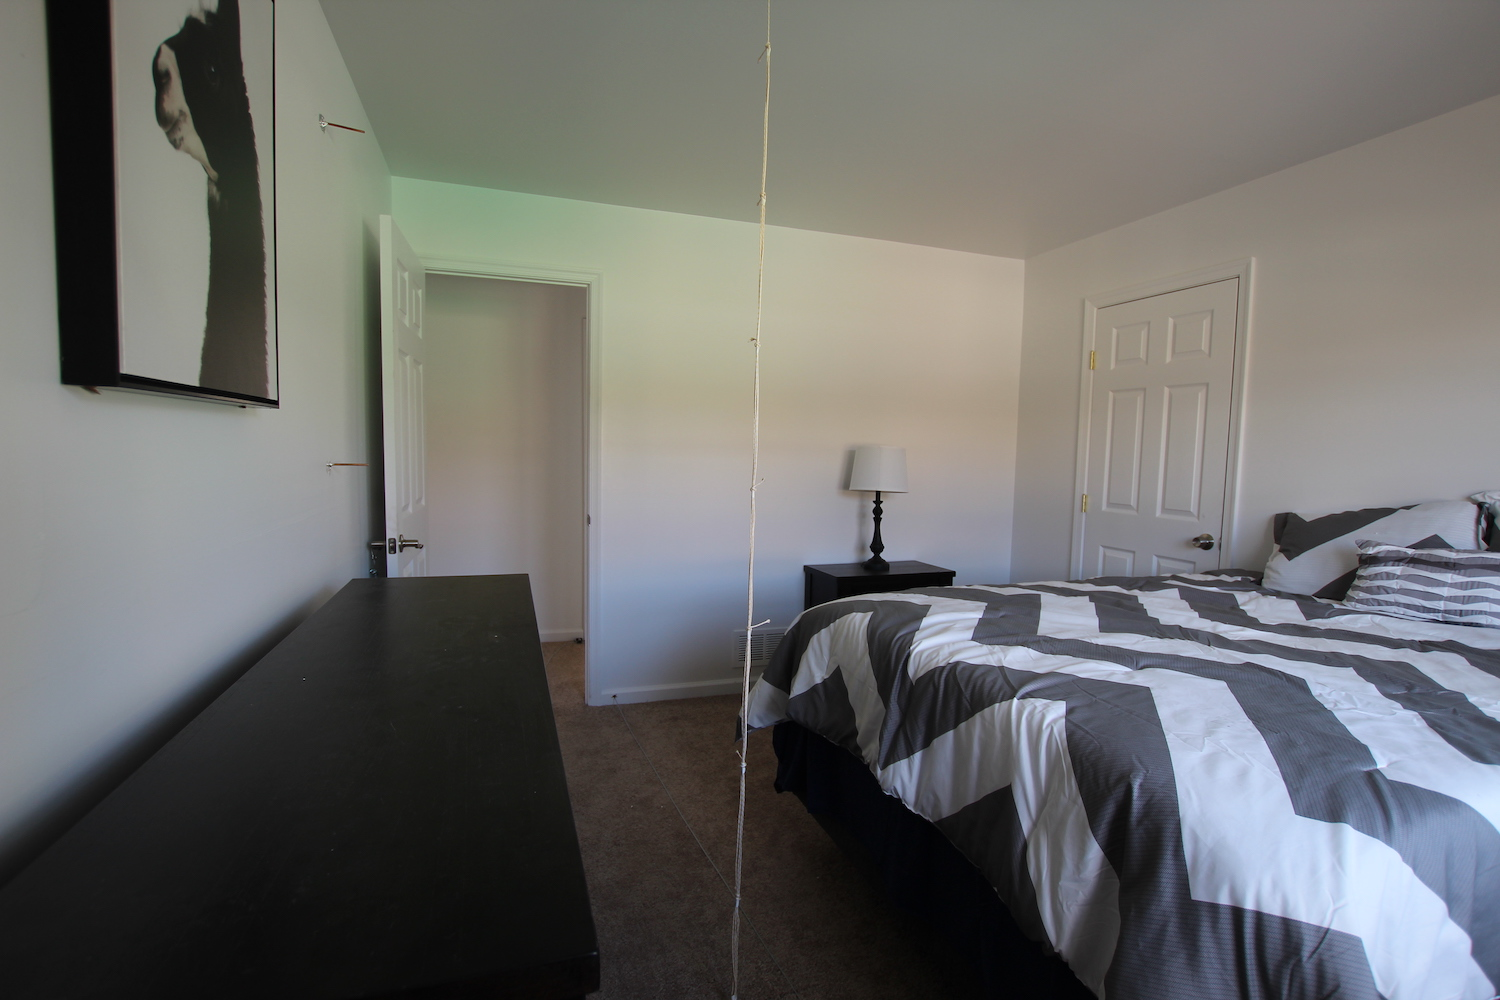
\includegraphics[width=0.49\textwidth]{../06_Figures/br_fuel_1.jpg}}\hfill
	\subfloat[View from Closet Toward Door and Windows\label{fig:br_fuel2}]{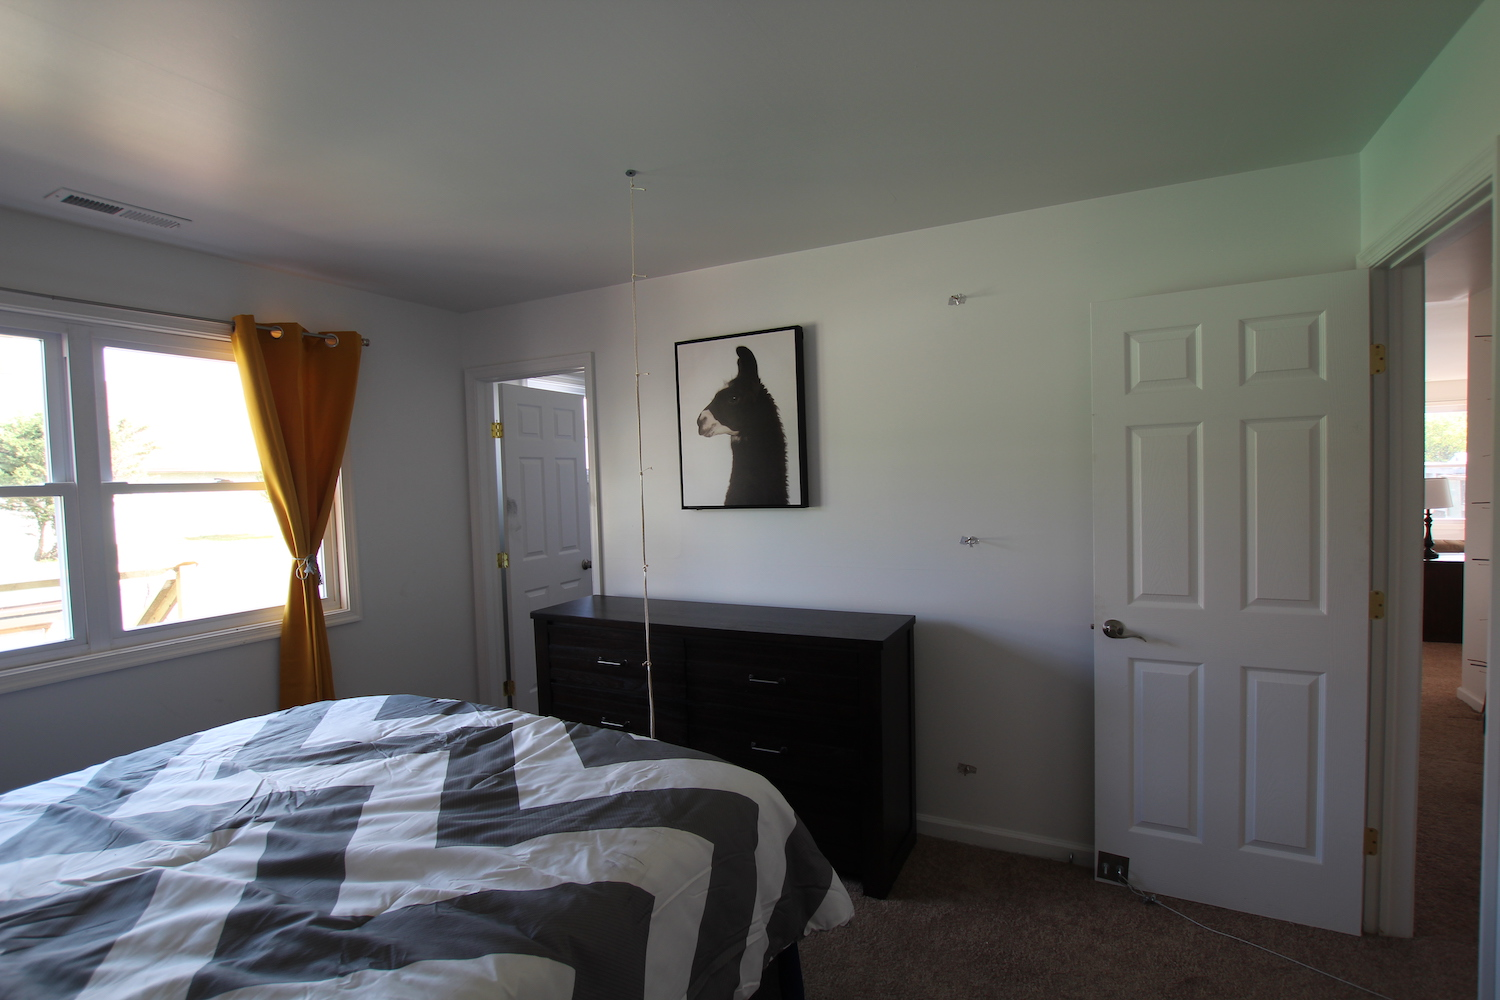
\includegraphics[width=0.49\textwidth]{../06_Figures/br_fuel_2.jpg}}\hfill
	\caption[Bedroom Fuel Photographs]{Typical layout of fuels in each bedroom.}
	\label{fig:br_fuel}
\end{figure}

\FloatBarrier



%Example of Figure Definition

% \begin{figure}[!ht]
% 	\centering
% 	\includegraphics[width=<set_width>]{<file_location>}
% 	\caption[Title of Figure for List of Figures]{Write the figure caption in sentence form. The caption should contain enough detail for the reader to thoroughly understand the figure. So, if the figure is a data plot, be sure to describe the meaning of the various line colors, styles, symbols, etc. used.}
% 	\label{fig:<ref_name>}
% \end{figure}


\chapter{Results \& Discussion}



\chapter{Research Needs}


\chapter{Summary}


\bibliography{UL_general,UL_FSRI,NFPA_std,NIOSH}

\clearpage

\appendix
\captionsetup{list=no}

\end{document}
